%%%%%%%%%%%%%%%%%%%%%%%%%%%%%%%%%%%%%%%%%%%%%%%%%%%%%%%%%%%%%%%%%%%%%%%%%%%%%
%%% PIA Tutorial
%%% Julian Uszkoreit
%%% julian.uszkoreit@rub.de
%%%%%%%%%%%%%%%%%%%%%%%%%%%%%%%%%%%%%%%%%%%%%%%%%%%%%%%%%%%%%%%%%%%%%%%%%%%%%

\pdfminorversion=4
\documentclass[a4paper,11pt,twoside]{article}
\usepackage[T1]{fontenc}
\usepackage[utf8]{inputenc}
\usepackage[onehalfspacing]{setspace}
\usepackage{changepage}
\usepackage{emptypage}
\usepackage{listingsutf8}
\usepackage{graphicx}
\usepackage[dvipsnames]{xcolor}
\usepackage[small,bf,margin=1cm,singlelinecheck=true]{caption}
\usepackage[a4paper]{geometry}
\usepackage{layout}
\usepackage{hyperref}
\usepackage[ddmmyyyy,hhmmss]{datetime}

% set font family
\usepackage{lmodern}
\sffamily %to load T1lmss.fd

% Load 'sans small caps' from helvet:
\usepackage{helvet}
\sffamily %to load T1phvss.fd
% Substitute non-existing lmss/bx/sc with phv/bx/sc
\DeclareFontShape{T1}{lmss}{bx}{sc} { <-> ssub * phv/bx/sc }{}
% Can also pick the sans small caps:
\DeclareFontShape{T1}{lmss}{m}{sc} { <-> ssub * phv/m/sc }{}

\renewcommand*\rmdefault{lmss}

% to nicely show menu entries
\newcommand{\menu}[1]{{\scshape\bfseries #1}}
% to nicely show files
\newcommand{\filepath}[1]{{\scshape\bfseries #1}}
% to nicely show kniem nodes
\newcommand{\knimenode}[1]{{\scshape\bfseries #1}}

% set date separator
\renewcommand{\dateseparator}{.}


\title{Tutorial of PIA -- Protein Inference Algorithms}
\author{Medical Bioinformatics\\
	Medizinisches Proteom-Center\\
	Ruhr University Bochum}


\begin{document}

%%%%%%%%%%%%%%%%%%%%%%%%%%%%%%%%%%%%%%%%%%%%%%%%%%%%%%%%%%%%%%%%%%%%%%%%%%%%
%%% TITLE PAGE
\thispagestyle{empty}
\begin{titlepage}
	\vspace*{\fill}
	\begin{adjustwidth}{-2cm}{-2cm}
		\begin{center}
			{\huge \textbf{PIA -- Protein Inference Algorithms\\
					Tutorial}\\[2cm]}
		\end{center}
	\end{adjustwidth}

	\begin{center}
		
\includegraphics[width=0.5\textwidth]{graphics/pia_logo_big}\\[2cm]

		{\large Medical Bioinformatics\\
			Medizinisches Proteom-Center\\
			Ruhr-Universität Bochum\\[0.5cm]}
		{\large https://github.com/mpc-bioinformatics/pia\\[0.1cm]}
	\end{center}

	\vspace*{2cm}
	\begin{center}
		Creation date \today{}, \currenttime{}.
	\end{center}
	\vspace*{\fill}
\end{titlepage}

%%%%%%%%%%%%%%%%%%%%%%%%%%%%%%%%%%%%%%%%%%%%%%%%%%%%%%%%%%%%%%%%%%%%%%%%%%%%

\tableofcontents
\newpage


\section{Introduction}

\subsection{PIA -- Protein Inference algorithms}

PIA is an open source toolbox for MS based protein inference and identification
analysis. As in bottom-up MS proteomics actually peptides are identified, but
most often the entities of interest are proteins, the protein content of an
analysed sample must be constructed from the knowledge of the contained
peptides. This step is known as "protein inference" and is the heart of PIA.
Furthermore, PIA can be used to inspect, analyse, perform quality checks
on and filter identified peptide spectrum matches (PSMs) and peptides. This can
be performed either via KNIME nodes or the command line. While the latter
method is intended for advanced scripting and the command line tools can now
also be downloaded as a Docker image, we will mainly discuss the usage of KNIME
nodes in this tutorial.


\subsection{Prerequisites}

All data and workflows can be downloaded in the tutorial repository at\\
\url{https://github.com/julianu/pia-tutorial}.

\begin{itemize}
	\item Knowledge of mass spectrometry based bottom-up peptide identification
	\item Basic knowledge of KNIME and constructing workflows with KNIME

	\item It is helpful to know the basics of OpenMS for KNIME, mainly the usage
	of spectrum identification nodes. For the advanced and quantification chapter,
	also the basics of quantification should be known. But both are also shortly
	sketched in this tutorial. (The OpenMS tutorial can be found at
	\url{http://www.openms.de/tutorials/})

	\item The tutorial was tested using the stable PIA 1.3.9 nodes and the stable
	OpenMS 2.3.0 nodes with KNIME 3.6.1
\end{itemize}

\subsection{Version}

This tutorial was created on \today{} at \currenttime{}.


\newpage
\section{Installation of PIA KNIME nodes}

If not yet done, you first need to download and install KNIME to your system
(\url{https://www.knime.com/downloads}). After installing KNIME, start up the
analystics platform and install the PIA nodes from the community contributions
repository. For this, go to \menu{Help > Install New Software...}. Select the
community contributions repository under the \menu{Work with} drop down menu, it
should contain an address similar to
\url{http://update.knime.org/community-contributions/trusted/3.6}. The PIA nodes
can be found in the \menu{Bioinformatics \& NGS} group or simply by searching
for them. Select the PIA nodes, click next, accept the license and restart KNIME
after the installation is finished.

If all went well, you will see the PIA octopus on the splash screen of KNIME
(together with all the other icons) and you will find the PIA nodes inside the
\menu{Community Nodes} in the Node Repository (usually left bottom side of
screen). This tutorial also needs the OpenMS nodes (also in the community
contributions' \menu{Bioinformatics \& NGS}, next to PIA nodes).


\newpage
\section{Basic PIA analysis in KNIME}

First download the workflows and data for the tutorial at
\url{https://github.com/julianu/pia-tutorial}.


\subsection{First workflow}

Import and open the workflow \filepath{01-PIA\_first\_analysis} from the
provided workflows into your KNIME workspace. First, we will run a minimal
workflow identifying spectra in an mzML file with the search engine X!Tandem
and using PIA for the protein inference and also analysis of the identified
PSMs and peptides. If you don't want to run the identification step, you can
skip it by pointing the \knimenode{Input File} node in the "skip
identifictaion" box to the idXML (\filepath{1a-QExHF04026.idXML}) and directly
go to \ref{pia_compilation}


\subsubsection{Spectrum identification}

Please select the file \filepath{1a-QExHF04026.mzML} as the input spectra file
(upper \knimenode{Input File}) and the provided FASTA file with decoys \\
(\filepath{uniprot-proteome-mouse-spiked-cRAP-iRT-isos-2017\_03-decoy.fasta})
as the database for spectrum identification. We will use X!Tandem for spectrum
identification in this workflow. If you like, you can change it to any other
supported spectrum identification software in KNIME or make the identification
externally e.g. with Mascot or Proteome Discoverer. But then, you need to load
the results directly into the \knimenode{PIA Compiler} node, for example by
using the \knimenode{Input File} also available to skip the identifications.
The basic configuration settings for spectrum identification of the files used
in the tutorial are:

\begin{itemize}
	\item 10 ppm precursor tolerance
	\item 0.02 Da fragment tolerance (or 20 mmu)
	\item tryptic digestion with up to 2 missed cleavages
	\item fixed Carbamidomethyl of C and variable Oxidation of M of modifications
\end{itemize}

The \knimenode{PeptideIndexer} is needed to add the protein / accession
information to the identified peptide spectrum matches (PSMs). For the tutorial
data, use "DECOY\_" as the decoy string and prefix as decoy position and make
sure that "Trypsin" is set as enzyme with "none" as specificity.


\subsubsection{PIA compilation}
\label{pia_compilation}

After adjusting the \knimenode{Input File} nodes, if wanted reconnecting the
the \knimenode{Input File} for skipping the identifications, and maybe checking
the other nodes' settings, run the workflow until the \knimenode{PIA Compiler}
by right-clicking on the node and selecting \menu{Execute}.

This node takes a list of files. Note, that the ports from OpenMS (blue squares)
need to be converted into a URI file list (black triangle, these represent the
common KNIME table data). You could alternatively use a \knimenode{List Files}
node to select the files containing prior performed spectrum identifications in
any supported format like Mascot Dat, X!Tandem's XML files, Proteome
Discoverer's MSF files or any mzIdentML file, and use these files as input for
the compiler. The \knimenode{PIA Compiler} is necessary to structure the data
before a PIA analysis. It must be performed only once per set
of identification files. The node has as configuration settings only a
compilation name, which can be chosen freely. The number of files passed to PIA
is not limited, though processing more files needs more main memory. Each file
in the compilation gets a FileID, which you can explore with some additional
information of the compilation when looking at the \menu{View: summary} after
running the \knimenode{PIA Compiler}. These IDs can also be used for filtering
and advanced settings later on.

\begin{figure}[ht!]
	\centering
	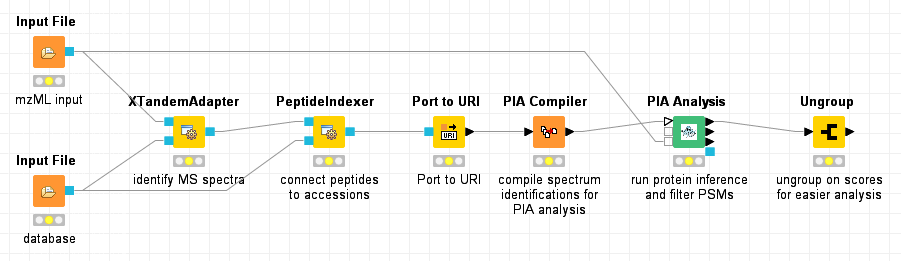
\includegraphics[width=\textwidth]{graphics/first_analysis_workflow}
	\caption{A basic protein analysis workflow using X!Tandem for spectrum
	identification and PIA for protein inference.}
\end{figure}

The first connected port of the \knimenode{PIA Analysis} node is for the PIA
compilation, directly coming from the compiler node. If you should have a saved
compilation, you could also load this with an \knimenode{Input File} node
together with the second input port. The first port of both with a suitable
configured file will be processed for analysis. The third input port is used to
pass spectrum data to PIA, which can be used to visualise automatically
annotated spectra. If you don't want to use the spectrum viewer, you should not
connect anything to this port. As the matching of the PSMs to their spectra
might take some time, you should consider using this only when you need a
spectrum annotation.


\subsubsection{General Settings}

After running the compiler, open the settings of the \knimenode{PIA Analysis}
node, either by double clicking on the node or right clicking and selecting
\menu{Configure...}. You will find four tabs for the settings: one general and
one for each of the three levels of analysis (i.e. PSMs, peptides and proteins).
If you connected the compiler node directly to the analysis node, select the
column containing the PIA XML file in the respective setting (there is mostly
only one named "gzipped PIA XML file"). You can also set, whether PIA should
fail if no decoys were found in the analysis, whether PSM sets should be created
and whether modifications should be considered to distinguish peptides (see
Figure \ref{pia_settings_general}). Creating PSM sets should always be used, if
the same spectrum file was analysed with different search engines. This option
will then combine the results of multiple searches. Otherwise, when e.g.
combining the results of multiple MS runs identified by only one search engine
or, like in the example workflow, having only one search engine for one file, it
can savely be deselected. Mostly, a peptide and it's scoring influence for the
proteins should only be described by its sequence. If you have stable
modifications, though, you can select to distinguish peptides by sequences and
modifications. The \knimenode{PIA Analysis} node allows to export the analysis
into several file formats. The level of the export (PSM, peptides and protein)
as well as the format can be selected appropriately. Currently only one export
file can be created at once.

\begin{figure}[ht!]
	\centering
	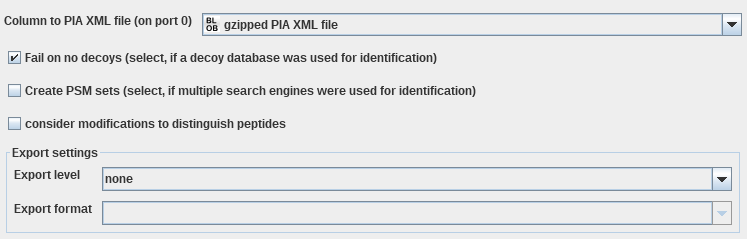
\includegraphics[width=0.9\textwidth]{graphics/pia_settings_general}
	\caption{The general settings dialog of the \knimenode{PIA Analysis} node.}
	\label{pia_settings_general}
\end{figure}

The analyses at the PSM and peptide level of PIA will be performed only for the
input file given by the FileID in the respective settings tab. Usually, the IDs
start with 1 and are sorted by the order of the given input files. A special
case is the combination of all runs (either with PSM sets or without), also
called overview, which has always the ID 0. The 0 for FileID is the default for
the PSM and peptide level analyses.


\subsubsection{PSM Settings}

Now, have a look at the PSMs settings of the \knimenode{PIA Analysis}. The
first setting is the just mentioned file ID, which is 1 in the example and thus
reflects the first file of the compilation (Note: we have only one file in this
example, but still 0 could be used for the overview, if e.g. you would like to
calculate the "Combined FDRScore". Then you would also need to enable the
creation of PSM sets and the calculation of the "Combined FDRScore". For one
single input file, though, this would be identical to the normal FDRScore).
Remember, you can check which file has which ID in the view of the compiler
node. Next you can choose to calculate the false discovery rate (FDR), and thus
also FDRScore and q-value, for all input files. The FDRScore \cite{jones2009}
smoothes the FDR q-values in an analysis and thus facilitates a better
discrimination of identifications instead of using the FDR q-values alone. If
PSM sets are created, also the Combined FDRScore can be calculated, which
furthermore allows the combination of search results from multiple MS runs as
well as identifications from different search engines.

\begin{figure}[ht!]
	\centering
	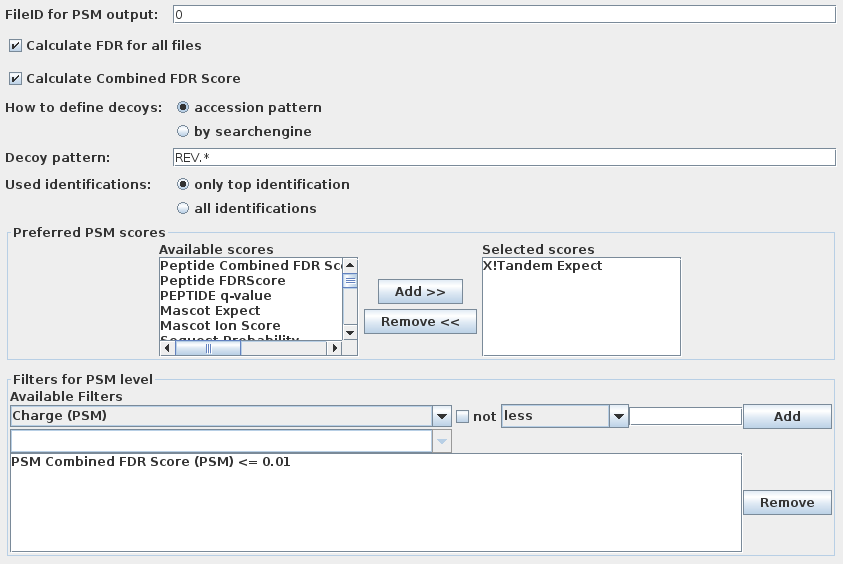
\includegraphics[width=0.9\textwidth]{graphics/pia_settings_psms}
	\caption{The PSMs settings dialog of the \knimenode{PIA Analysis} node.}
	\label{pia_settings_psms}
\end{figure}

A very important step is the selection of how decoys are distinguished from
target identifications. PIA allows to use regular expressions for this, which
are applied to the accessions. In the example in Figure
\ref{pia_settings_psms}, "DECOY\_.*" is set as regular expression. So each
accession starting with the string "DECOY\_" (and all its peptides) will be
assigned to be decoys and all not matching accessions to be targets.
Alternatively, if "by search engine" is selected, identifications must be
annotated in the input files as targets and decoys. This is e.g. the case if in
Mascot the "Decoy" option is selected for an MS/MS search. For better
compatibility though, the usage of a target-decoy database and the assignment
by regular expressions is recommended. For this to work, don not filter the
identifications for decoys or FDR before passing them to PIA.

Some search engines report more than one identification per spectrum. In the
next option, you can choose to either use all these identifications or only the
one with the best score for the FDR analysis and all following steps. Finally,
you can select which scores are used for FDR estimation. If a search engine
reports multiple score (e.g. X!Tandem's Hyperscore and Expect), you can choose
the preferred score here. If no score was chosen, PIA will use the main score of
the search engine (or, if this was not given, just any score, but this
consistanly).

All the settings up to this point are used for the FDR calculation (except for
the output file ID) and influence the peptide and protein reports as well. The
filters though afflict only the PSM level and its report. Here you can chose
from the available filters and set the parameters accordingly. For score filters
it is necessary to select the according score as well in the line below the
actual filters selection. After selecting a filter and setting the parameters,
don't forget to click \menu{Add}. The currently activated filters will be shown
in the list. In the example workflow, a filter for the "PSM FDRScore <= 0.01" is
set. Keep in mind, that all filters have to be fulfilled for a PSM to pass the
filters (the filters are additive).


\subsubsection{Peptides Settings}

Next, select the peptides settings. All settings here are only relevant for the
peptide export and do not afflict the protein inference. Therefore, you can also
turn the peptide inference off and will get an empty reporton the peptide level.
This might be a good idea, if you want to save time and main memory during the
analysis. The selection of the file ID has the same meaning as on the PSM level:
exporting only information of the given file, or 0 for the combination of all
results. Again: if in doubt, check the file ID at the compiler view. Also the
filters are used in the same way. An exception are the PSM level filters: with
these, the PSMs which are actually used to create peptides, are filtered before
the epptide inference. In the example workflow and in Figure
\ref{pia_settings_peptides}, only PSMs with "PSM FDRScore <= 0.01" are inferred
to peptides, all other PSMs are discarded.

\begin{figure}[ht!]
	\centering
	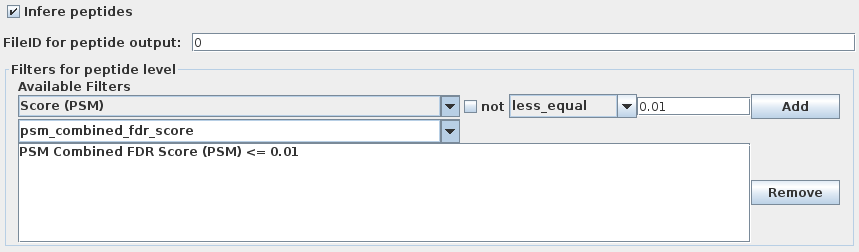
\includegraphics[width=0.9\textwidth]{graphics/pia_settings_peptides}
	\caption{The peptides settings dialog of the \knimenode{PIA Analysis} node.}
	\label{pia_settings_peptides}
\end{figure}


\subsubsection{Protein Inference and Protein Settings}

Finally, take a look at the proteins settings. Also the protein inference can
be turned off, if you are only interested in analyses on the PSM or peptide
level. First, you have to chose an inference method. PIA provides you with
three different methods (for a more thorough explanation of these methods,
please refer to \cite{uszkoreit2015})

\begin{itemize}
	\item \textbf{Occam's Razor} is based on the parsimony principle and
	returns the smallest set of proteins, which explain all identified
	peptides. This is a very widely used strategy for protein inference.

	\item \textbf{Spectrum Extractor} is the recommended method. It is also
	based on the parsimonious approach, but assigns a spectrum to only one
	peptide. These peptides are selected in such a way, that they increase the
	score of the most probable, possible protein group.

	\item \textbf{Report All} This strategy reports all possible protein groups,
	based on the given data. Use this with caution and only when you know, what
	you are doing! It's mainly used when searching for a special protein group in
	your data.
\end{itemize}

\begin{figure}[ht!]
	\centering
	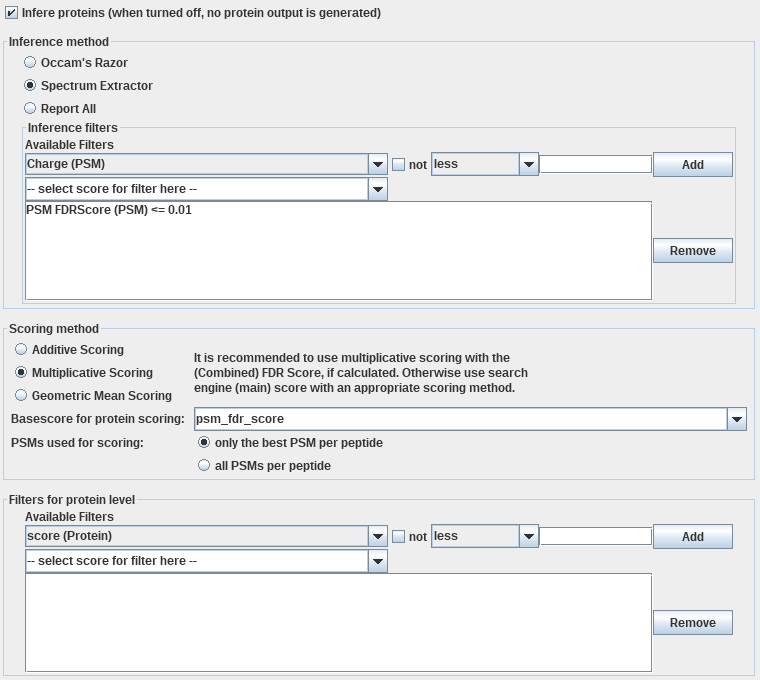
\includegraphics[width=0.9\textwidth]{graphics/pia_settings_proteins}
	\caption{The proteins settings dialog of the \knimenode{PIA Analysis} node.}
	\label{pia_settings_proteins}
\end{figure}

After selecting the inference method, you can apply a variety of filters, which
will be applied on PSM, peptide and protein level and directly afflict the
results of the inference. You should almost always filter on the PSM level FDR,
either using the FDR Score or the Combined FDR Score, usually on a value of about
0.01. Remember: if you searched with only one search engine, the FDR Score will
be the score of choice, for multiple search engines the Combined FDR Score. But
you could also set filters which allows only protein groups with at least two
peptides, and many more filters.

Next, you need to select the scoring method. Here, you should use "additive
scoring" only if your base score has a "higher score is better" probability,
like e.g. the Mascot Ion Score or X!Tandem's Hyperscore. Otherwise, use one of
the other two scorings. The "multiplicative scoring" takes the number of
identified peptides into account, in the way that the final protein score is
usually better with more distinct peptides. The "geometric mean scoring" on the
other hand calculates the mean of all peptide scores.

Finally, you need to select the base score and whether only the best PSM
(recommended) or all PSMs of a peptide should be used for scoring. In our
example, the FDR Score is used. Note: As base score you can only
select scores on the PSM level, as the peptides will be generated during the
inference according to your applied filters.

The protein report can also be filtered in the same way as the PSMs and
peptides report. Be aware, that this is significantly different to setting an
inference filter on protein level: filters applied for the inference make it
possible to not even create a protein group. Filters on the protein report
afflict only what will be reported, not what will be inferred.


\subsubsection{A word on filters}

Though PIA provides you with many filters on each of the PSM, peptide and
protein level, you can also apply these filters later in the workflow. For
this, you can simply apply an appropriate \knimenode{Row Filter} node after
running the \knimenode{PIA Analysis}. But also keep in mind that setting the
inference filters on the protein level are behaving very differently, as
explained in the prior paragraph.


\subsection{Looking at the Results}

Now run the \knimenode{PIA Analysis} node. This will, depending on the loaded
data, take some time. The example data should be processed in a few minutes
though. The node has four output ports: the first two are the (filtered)
reports on the PSM and peptide level for the selected input file, the third is
the protein level report and the last is a file port for the exported data, if
any was created according to the settings in the general settings tab.


\subsubsection{Analysis Viewer}

To explore the results of the analysis, right click on the \knimenode{PIA
Analysis} node after the execution finished and select the \menu{View: PIA
Results Analysis}. In the top left corner you will see all the inferred protein
groups. PIA always works with protein groups, even if such a group might
contain only one accession. All the accessions in one group have exactly the
same evidence, i.e. the same PSMs and peptides, and cannot be distinguished on
the given data and applied inference settings, at least without any further
knowledge. The score is calculated using the selected base-score and scoring
method. A higher score is always better (for base scores with "lower score
better" a -log value is used for transformations). If the complete protein
sequences were provided, the coverages for the proteins are calculated.
Furthermore, the number of assigned spectra, PSMs and peptides are listed next
to these. If the FDR was calculated, also the decoy status and the protein level
FDR q-value is given.

\begin{figure}[ht!]
	\centering
	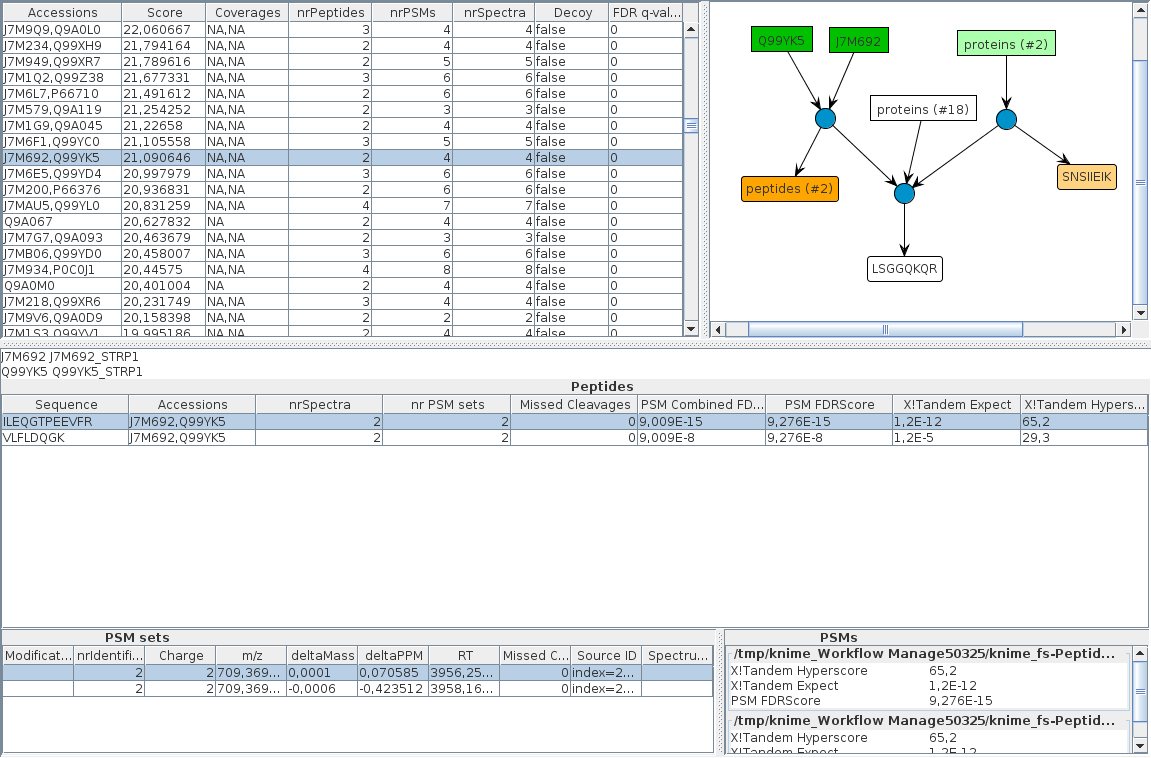
\includegraphics[width=0.9\textwidth]{graphics/screenshot_PIA_analysis}
	\caption{The PIA analysis viewer allows an intuitive exploration of the
	data.}
	\label{pia_analysis}
\end{figure}

For the currently selected protein group, the assigned peptides (i.e. the ones,
that were not filtered out by the inference filters) are listed together with
their information in the central list of the window. On the bottom left, all
PSM sets of the currently selected peptide are listed and on the bottom right
finally the individual PSMs are given. If the corresponding spectrum file was
passed to the analysis node, you can view the annotated spectrum when clicking
on the button by the PSM (see also PSM Results).

On the top right you will see a directed graph showing the relations between
accessions of the currently selected protein group and its peptides and PSMs.
This might look a bit overwhelming at first, but can be helpful, if you know
how to read it. In the example workflow, take a look at the group "P02675" (it
has a score of 71.71) and "Q91V41" (score of 20.13). The accessions of the
selected group are coloured in dark green with a black border. Accessions of
(not reported) sub-groups are given in light-green without border and accessions
reported in other groups in light green with black border. Peptides are coloured
in orange (dark for the selected group, light for other groups in the same way
as accessions). The blue circles are drawn only to construct a correct tree.
Nodes which hold multiple items, can be expanded by double clicking on them, as
can peptides to show their corresponding PSMs. All items can be re-arranged by
drag-and-drop.


\subsubsection{PSM Results}

To look at the PSM level report-table, right click on the \knimenode{PIA
Analysis} node and select \menu{0: PSM results}. In this table you have almost
all available information for the PSMs, like the amino acid sequence, a list of
accessions, modifications, precursor charge, m/z value, the mass error, etc.
Also, you have three columns for the scores (scores, score names and score
shorts), which are lists each. Here, the score on a given position in the list
corresponds to the score name and its short (which is an abbreviated name) on
the same positions in the list. This makes it possible to export multiple scores
in one row. In our example, we have three different scores per PSM: the
X!Tandem Hyperscore and Expect, as well as the FDR Score.

For easier analysis, the scores can be ungrouped using the \knimenode{Ungroup}
node on the PSM report, which is the second last step in the workflow. Take a
quick look at the \knimenode{Ungroup}'s settings and verify, that it is set to
ungroup on the three score columns (and not the accessions). Run the node and
look at the results: the score columns contain now individual names and
numbers, which can be used for further sorting and filtering. Note also, that
there is three times the number of rows after the ungrouping. To leave only the
PSM FDR Score in the table, the final \knimenode{Row Filter} is used.

An alternative, though not that comprehensive way to look at all reported PSMs
(but not any PSM sets) is using the "PSM Spectrum Viewer". Here you can see the
PSMs together with the automatically annotated spectra (using \cite{perez2015}).
This only works, if you connected the identified spectrum file to the third
PIA input port.

\begin{figure}[ht!]
	\centering
	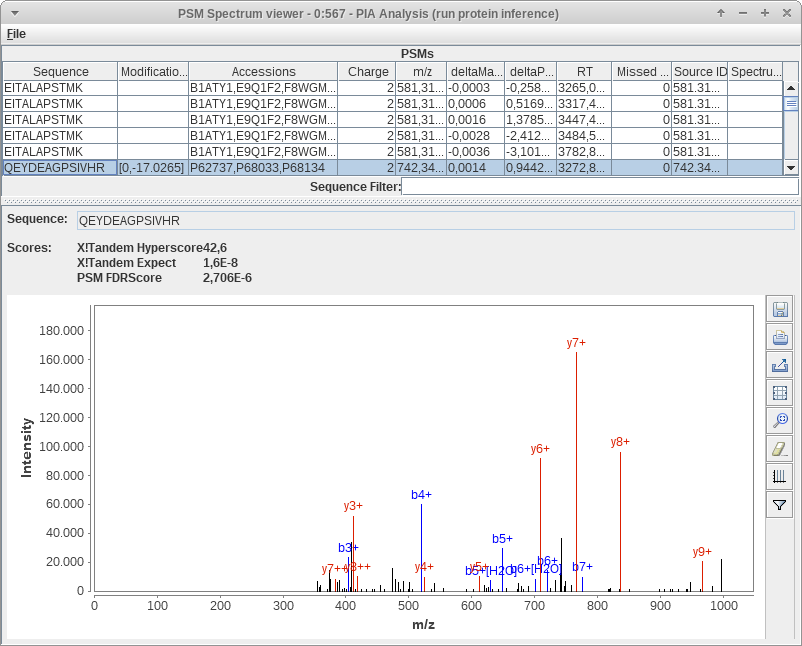
\includegraphics[width=0.9\textwidth]{graphics/screenshot_PSM_spectrum_viewer}
	\caption{The PSM spectrum viewer showing an automatically annotated
	spectrum.}
	\label{pia_psm_spectrum_viewer}
\end{figure}


\subsubsection{Peptide Results}

The peptide results are given in the same way as the PSM results. The peptides
are inferred either with or without taking modifications into account, as
explained before.


\subsubsection{Protein Results}

The created protein table on the third port holds almost the same information
as the table in the \textbf{PIA Result Analysis} view. Node, that the accessions
are lists again, as PIA always reports protein groups. Additionally, each group
has a clusterID, which represents the connected set or tree in the PIA
intermediate structure. Elements in such a cluster are connected by their
relations of accessions and PSMs, as can be seen in the \textbf{PIA Result
Analysis} view on the top right. This does not mean, that reported protein
groups with the same cluster ID share a peptide, but they are in the same
component (a tree in the top right region of the \textbf{PIA Result Analysis}
view) and can be connected by other (even not reported) accessions or peptides.

All of the reported tables can easily be processed with default KNIME nodes.
This facilitates filtering, sorting, plotting etc. But also an analysis with R
or Python can be created without much effort. If you like, you can also export
the tables to excel and process them further.


\subsubsection{The Export File Port}

On this port the created export file can be found. This could be either used
to create an mzIdentML or mzTab file for storage and uploading into e.g. the
PRIDE repository, but also as input for OpenMS's \knimenode{ProteinQuantifier},
if an idXML file was exported (as shown in the advanced tutorial).
Additionally, you could create CSV files for usage in downstream processes or
manual inspection.


\subsection{Tasks}

\begin{itemize}
	\item Find the protein group "P02675" in the \textbf{PIA Results Analysis}
	view (it has a score of 71.71). Try to understand, why this protein (group)
	was reported, but no group with Q8K0E8 was reported.

	\item Now find find the protein group "Q91V41" (score 20.13). Why
	was this group and also the group "P62821, Q5SW88, Q9D1G1" (score 6.07)
	reported, which has shared peptides?

	\item Make a PIA analysis of the same data, but use an additional search
	engine. For this, you should activate the creation of PSM sets and set the
	used inference base score to the Combined FDR Score.\\
	Hint: The workflow for this is given in the data folder, but try to extend the
	workflow on your own first. ;)
\end{itemize}



\newpage
\section{PIA for inference of quantitative data}

PIA can be used for protein inference on quantitative data. For this, PIA can be
allows to infere the protein groups and facilitate a quantification, which is
not dependend on unique peptides. This is achieved due to the fact, that PIA
groups the proteins, which have the same evidence, into a protein group. Be
aware, though that protein-subgroups are not represented by this at the moment.

The inference for quantification works out of the box with PIA and OpenMS. A
workflow showing this on a small dataset (just load in the provided files) is
given in the data folder of this tutorial.

First you need to run a feature detection, map IDs, align and normalise
the data to create a featureXML. More about these steps can be found in the
OpenMS tutorial. Then, you can use PIA to create the inference input for the
\knimenode{ProteinQuantifier}. For this, you just need to select idXML and
protein level as export in the general settings and run the
\knimenode{PIA Analysis} node. The settings should be applied with respect to
the provided data. All information for this can be found in the prior chapter.

\begin{figure}[ht!]
	\centering
	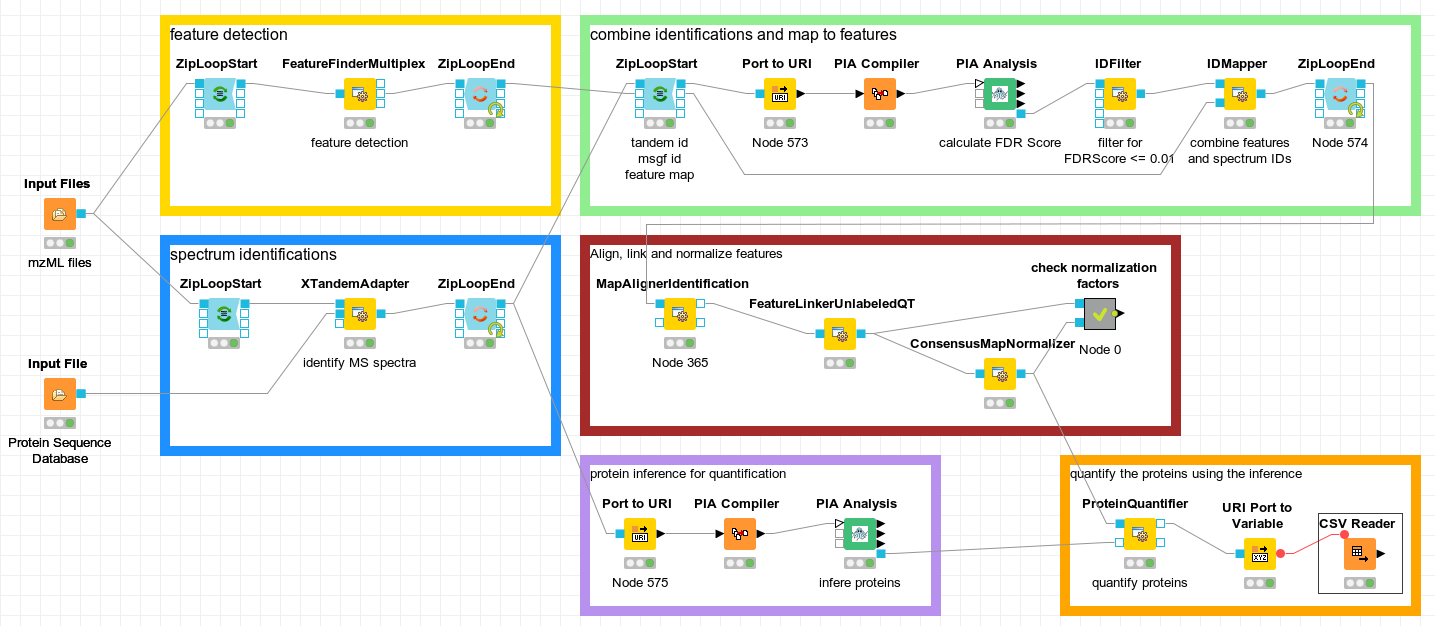
\includegraphics[width=0.9\textwidth]{graphics/quant_workflow}
	\caption{A basic workflow using PIA for the protein inference used for
	protein quantification.}
	\label{quant_workflow}
\end{figure}

\subsection{Tasks}

\begin{itemize}
	\item Run the provided workflow on the small test dataset. Verify, that\\
	"P68871/contaminant\_HBB\_HUMAN" is a valid candidate for a regulated protein.
\end{itemize}



\newpage
\section{Web Frontend}

The Docker execution is not yet explained here. To install the Docker image,
you only need the following command:

\begin{verbatim}
	docker pull biocontainers/pia
\end{verbatim}

Further documentation will follow. For now, take a look at the PIA wiki at
GitHub for how to use the command line interface.


%% TODO: add more docker information


\newpage
\begin{thebibliography}{9}
	\bibitem{uszkoreit2015}
	Uszkoreit et al.,
	\emph{PIA: An Intuitive Protein Inference Engine with a Web-Based User
	Interface.},
	J Proteome Res,
	2015.

	\bibitem{jones2009}
	Jones et al.,
	\emph{Improving sensitivity in proteome studies by analysis of false
	discovery rates for multiple search engines.},
	Proteomics,
	2009.

	\bibitem{perez2015}
	Perez-Riverol et al.,
	\emph{ms-data-core-api: an open-source, metadata-oriented library for
	computational proteomics.},
	Bioinformatics,
	2015.
\end{thebibliography}

\end{document}
